\chapter{Literature study}\label{chapter:literature_study}

% introduction to the literature study

This chapter describes the various components that are used in the development of this thesis. Section \ref{chapter:literature_study:section:computer} looks at recommender systems and their rationale. Next we will look at visualization techniques and how these can be used to visualize the recommendation rationale in section \ref{chapter:literature_study:section:interaction}. After this, insight gaining and human perceptual skills are investigated in section \ref{chapter:literature_study:section:user}. We discuss how insight gaining can be evaluated and how the user is expected to use the visualization in a visual thinking algorithm. Finally we discuss and compare other visual explanation systems in section \ref{chapter:literature_study:section:applications}.




% -------------------------- The System ---------------------------
% 
% -----------------------------------------------------------------
\section{Recommender systems}\label{chapter:literature_study:section:computer}

A recommender system\index{recommender system} is a system that computes item suggestions for users based on a ratings of related items in the user's profile and/or history. Additional information can be incorporated into the recommendation algorithm\index{recommendation algorithm} to refine suggestions. Several categorizations of these techniques are proposed in literature \cite{bostandjiev:2012, burke:2002, herlocker:2000, melville:2002:CCF:777092.777124, celma:2008:phd}.

One of the incentives behind creating recommender system is the 'long-tail phenomenon'\index{Long Tail}\cite{rajaraman:2012}. This phenomenon can be explained as follows. Physical retail and warehouses can only keep a subset of all the available items in stock. These items are usually the most popular items on the market. Online vendors however, such as \emph{Amazon}\footnote{\url{http://www.amazon.com/}}, can offer a vastly larger subset of these items to clients, including also less popular and/or less known items\cite{rajaraman:2012}. Typically the long-tail phenomenon is visualized in a graph in which items are ordered by their popularity on the horizontal axis against the popularity rating on the vertical axis, as can be seen on figure \ref{figure:longtail}. Physical stores will offer only items in the first part of the graph, whereas the online vendors will also sell items from the remaining 'long tail' of the graph\cite{rajaraman:2012, celma:2008:phd}. Recommender systems then provide a means to find relevant items within this much larger range of items\cite{rajaraman:2012}. They enable to "connect supply and demand, introducing consumers to these new and newly available goods and driving demand down the tail "\cite{anderson:2006:LTW:1197299, celma:2008:phd}.

\begin{figure}%
	\begin{center}
		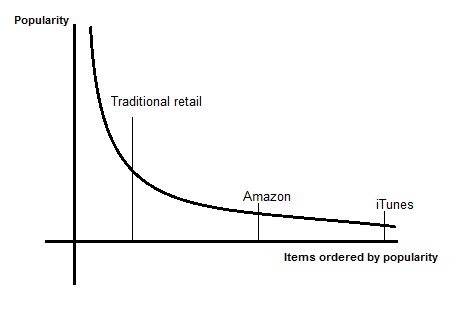
\includegraphics[width=250px]{img/longtail}%
	\end{center}
	\caption{The long-tail: Items ordered by popularity are layed out against their popularity rating. Most of the items reside in the long tail of the graph. Companies such as Amazon can offer a vastly greater subset of the total item space.}%
	\label{figure:longtail}%
\end{figure}

Typical applications of recommender systems are product recommenders for online retailers, movie and music recommenders such as \emph{Netflix}\footnote{\url{http://www.netflix.com/}} and \emph{Last.fm}\footnote{\url{http://www.last.fm/}}, and news article recommenders in online news services\cite{levy:2010, rajaraman:2012, celma:2008:phd}.


\subsection{Properties of recommender systems}\label{chapter:literature_study:section:computer:subsection:properties}

In \cite{herlocker:2004:ECF:963770.963772} and \cite{shani:2011:9780387858197}, Herlocker et al. and Shani et al.  respectively, compare the performance of recommender systems. A number of metrics for recommendation algorithms are described among which the following properties are listed. We will also describe methods for testing these properties, as described in \cite{shani:2011:9780387858197}.

\begin{itemize}
	\item \textbf{Accuracy}: The accuracy of item recommendations. There are three broad classes of prediction accuracy measures:
	\begin{itemize}
		\item the prediction of the rating given by a user;
		\item the prediction whether or not a user will actually use the item (for example adding to a queue) opposed to predicting the rating itself;
		\item the prediction of a ranking among items rather than an explicit rating of each item independently.
	\end{itemize}
	This kind of property is typically tested through an offline test on a training set, where parts of the recorded user profiles are hidden. The accuracy of the recommender system can then be determined by comparing the found recommendations to the remainder of the user profiles.
	\item \textbf{Novelty}: Novel recommendations are recommendations for items that the user did not know about. In a user study, users can be asked whether or not recommendations were new to them.
	\item \textbf{Serendipity}: Serendipity is a measure of how surprising the successful recommendations are. One can think of serendipity as "the amount of relevant information that is new to the user in a recommendation, or alternatively as deviation from the 'natural' prediction"\cite{shani:2011:9780387858197}. Serendipitous recommendations usually carry a higher risk, as they fall further from the class of known preferences. To find out the serendipity of recommendations, users can be asked directly if the recommendation was unexpected.
	\item \textbf{Diversity}: Diversity is generally defined as the opposite of similarity. To measure diversity content-based approaches can be used that compare recommended items.
	\item \textbf{Coverage}: One way to define coverage is the percentage of all items that are recommended to users during an experiment. Note that the cold start problem relates to coverage as it measures the coverage for a specific type of users, namely new users.
\end{itemize}

Many of these properties are closely related, as diverse recommendations that have a high coverage are likely to be serendipitous and novel. Also tradeoffs exist between properties; for example accuracy may drop as recommendations become more diverse\cite{shani:2011:9780387858197}. Looking at the Long-tail phenomenon, coverage, serendipity, novelty and diversity tend to be important. In the context of music recommendation, users usually want to find new music\cite{levy:2010}.


\subsection{A classification of recommendation algorithms}\label{chapter:literature_study:section:computer:subsection:algorithms}

Based on classifications presented in \cite{burke:2002} and \cite{celma:2008:phd}, a categorization of different types of recommendation strategies can be identified. We will only discuss the two most prominent ones, namely collaborative filtering (CF)\index{recommendation algorithm!collaborative filtering} and content-based filtering (CB)\index{recommendation algorithm!content-based filtering}\cite{herlocker:2000, rajaraman:2012}, and list some hybrid strategies. In the literature on recommender systems other general approaches that are commonly identified, are utility-based filtering, knowledge-based filtering, demographic filtering, and expert-based filtering\cite{bostandjiev:2012, burke:2002, song:2012}.


\subsubsection{Collaborative recommendation}\label{chapter:literature_study:section:computer:subsection:algorithms:subsubsection:cf}

\emph{Collaborative recommendation}\index{collaborative recommendation|see{collaboratibe filtering}} aggregates item ratings by users. By establishing overlaps between ratings in the corresponding user profiles, the system generates new item recommendations\cite{burke:2002, herlocker:2000}. User profiles consist of a vector of items and their ratings, which are continuously updated as the user interacts with the system over time\cite{burke:2002}.

For CF-based recommendation\index{CF|see{collaborative filtering}}, there are two classes of entities: users $U$ and items $I$. The data itself can then be represented by a utility matrix\index{utility matrix} $A$. The entries $a_{i,j}$ of the utility matrix represent what is known about the degree of preference of user $u_{i}$ and item $i_{j}$\cite{rajaraman:2012}. As can be seen in figure \ref{figure:utilitymatrix}, the utility matrix will have many blanks as well. The goal of the recommendation algorithm is then to fill in the blanks\cite{rajaraman:2012}.

\begin{figure}%
\begin{center}
	\includegraphics[width=250px]{img/utility_matrix}%
\end{center}
	\caption{The utility matrix $A$.}%
	\label{figure:utilitymatrix}%
\end{figure}

% Similarity / distance functions ...
In order to calculate the blanks, there is a variety of similarity functions that has been developed, e.g. \emph{cosine distance}, \emph{Pearson correlation}, \emph{Tanimoto-Jaccard}\cite{Verbert:2011:DRI:2090116.2090122}. For example, a small cosine distance will most likely correspond to a high similarity between profiles\cite{rajaraman:2012}. The discussion of the mathematics behind each of the algorithms is beyond the scope of this thesis.


\subsubsection{Content-based recommendation}\label{chapter:literature_study:section:computer:subsection:algorithms:subsubsection:cbf}

\emph{Content-based recommendation}\index{content-based recommendation|see{content-based filtering}} learns a profile of the user's interests based on the features present in objects the user has rated. New recommendations can then be generated based on a similarity function on these features\cite{burke:2002, pazzani:2007:CRS:1768197.1768209}.

When applying content-based filtering, the choice of similarity or classification function will have a significant impact on the quality of the recommendations. More importantly though, is the choice of features. To ensure good performance, these features should also be extracted easily from large quantities of data.

Depending on the type of item that is being recommended, different approaches can be applied to extract features and construct \emph{feature vectors}\index{feature vector}. Textual information is often extracted using a technique called \emph{stemming}\index{stemming} that uses root forms capturing a common meaning behind groups of words. Tuples of root forms and \emph{TF.IDF}, i.e., term frequency times inverse document frequency\index{TF.IDF}\index{term frequency times inverse document frequency|see{TD.IDF}}\nomenclature{TD.IDF}{term frequency times inverse document frequency} scores are computed for each word\cite{pazzani:2007:CRS:1768197.1768209, rajaraman:2012}. The words with the highest scores are the words that characterize the document\cite{rajaraman:2012}. A downside of stemming is that the process may cause the loss of contextual information for each word\cite{pazzani:2007:CRS:1768197.1768209}.

In \cite{bostandjiev:2012} and \cite{melville:2002:CCF:777092.777124} web crawlers are used to gather and extract features from online documents. Each property or feature is a 'bag of words'\index{bag of words} that can be used in a naive Bayesian text classifier\index{Bayesian classifier}. This way each item can be categorized and the profile can be 'learned'\cite{melville:2002:CCF:777092.777124}.

\emph{Tags}\index{tag} are very useful as well. Although they can be generated from text, for complex objects such as images and music, tag generation relies on user input\cite{rajaraman:2012}. Nonetheless, emerging technologies such as the 'search by image' option introduced by \emph{Google}\footnote{\url{http://www.google.be/imghp?hl=nl&tab=Ti}}, allow to retrieve web sites, documents and key words related to the given image\cite{google:2011:afbeeldingen}.

Mathematical models for music also allow for feature extraction. Algorithms have been developed to classify music based on content features\cite{Li:2006:TIM:2219090.2219562, tzanetakis:2002}. There are various types of acoustic features that can be extracted. In \cite{Li:2006:TIM:2219090.2219562} a distinction is made between rhythmic content features, pitch content features and timbral content features.


\subsubsection{Hybrid recommendation}\label{chapter:literature_study:section:computer:subsection:algorithms:subsubsection:hf}

\emph{Hybrid filtering}\index{hybrid filtering} combines two or more recommendation algorithms\cite{burke:2002}. In \cite{burke:2002} a number of hybrid recommendation strategies are discussed. Robin Burke lists seven different approaches for combining recommendation algorithms. Each of these combinations also has its advantages and disadvantages. Not necessarily all combinations will be successful, and not all of them have been implemented\cite{burke:2002}.

A good hybrid model is likely to outperform any single approach, as weaknesses of one strategy may be cancelled out by the advantages of another\cite{song:2012}.

%Hybrid systems for music recommendation can be built that use both collaborative filtering approaches and content-based approaches.



\subsection{Challenges for recommender systems}\label{chapter:literature_study:section:computer:subsection:challenges}

Each recommendation technique has benefits as well as drawbacks. Some of these apply to all or most types of recommendation strategies, while others are only relevant to certain cases.

The \emph{cold start} and \emph{gray sheep} problem both affect prediction accuracy. The \emph{black box} problem is more closely related to perceived accuracy and trust in the recommender system.


\subsubsection{Cold start}

Both CF and CB-based recommendation algorithms suffer from the ramp-up\index{ramp-up|see{cold start}} problem in one way or the other. The 'ramp-up' or 'cold start' problem\index{cold start} (although they may refer to slightly different problems depending on the literature) is dual problem that encompasses two distinct, yet related problems as defined in \cite{burke:2002}:

\begin{itemize}
	\item \textbf{New User}\index{cold start!new user}: Finding recommendations for users with a limited rating history is hard. Since user profiles tend to build up over time, new users usually fall in this category. As a result, recommender accuracy tends to be lower for new users.
	\item \textbf{New Item}\index{cold start!new item}: A new item will most likely not have that many ratings associated with it, and as a result will not be easily recommended. This 'new item problem' typically emerges when new items are constantly added to the system; for example when browsing a constant stream of news articles. When new articles are introduced, not many users have had the chance yet to rate these items. In the case of a news feed, an additional problem is that these items are short-lived, meaning that at some point these item profiles will most likely stop receiving any ratings at all.
\end{itemize}

Both of these issues translate themselves into a sparse regions in the utility matrix. It is worth noting that content-based recommendation algorithms suffer less from the \emph{new item} problem, as these tend to rely on features that are inherent to the items themselves, rather than user generated content. This is one of the reasons hybrid approaches can provide a solution to collaborative filtering\cite{burke:2002}. For example, in \cite{melville:2002:CCF:777092.777124}, content-based predictors are used to create pseudo-user ratings to reduce sparsity of the utility matrix, used in a collaborative algorithm.


\subsubsection{Gray sheep}

A problem that is typical of collaborative filtering is the 'gray sheep problem'\index{gray sheep}\cite{burke:2002, herlocker:2000}. The gray sheep problem occurs when a user falls between different clusters of users that may have contradicting item ratings. As a result, it is hard to determine how to classify the user\cite{burke:2002}.

Classifying users is typically a harder problem than classifying artists. An artist can usually be classified into one particular genre, whereas two users may have one genre in common, but may have rather conflicting tastes as well\cite{rajaraman:2012}.

% Having a lot of users will increase the likelyhood of finding similar users, even if a user has a broad taste. \emph{IMDb}\footnote{http://www.imdb.com} shows statistics of similar users, and \emph{Last.fm} allows to browse neighbouring profiles.


\subsubsection{Black box}

Another issue with recommendation systems is that these system often appear as 'black boxes' towards the end user\index{black box}. The complexity of the algorithms used, prevents the user from understanding the recommendation rationale\cite{zhao:2010}. This problem may decrease the acceptance by the user of item suggestions. One of the solutions for this problem, proposed by Herlocker et al. in \cite{herlocker:2000}, is to provide an explanation system, i.e., the white box\index{white box}, on top of the recommender system that explains the recommendation process. This can be done through providing a transcript of the system's reasoning or through visualizations\cite{herlocker:2000}.

In this thesis we will focus mainly on this problem. We will look at the black box problem in the context of collaborative music recommendation, and try to design, implement and test a new visual explanation system in an effort to overcome this problem.


\subsection{Music recommendation}\label{chapter:literature_study:section:computer:subsection:music}

%A number of popular recommender systems for music exist. For example Last.fm, Spotify, Grooveshark, Deezer are specifically aimed at music recommendation, but also websites such as Facebook, Youtube, and Amazon have can provide recommendation for music. Most of these systems use collaborative filtering, sometimes in combination with content-based features.

\subsubsection{Examples}

A number of popular recommender systems for music exist, such as \emph{Last.fm}\footnote{\url{http://www.last.fm/}}, \emph{Spotify}\footnote{\url{http://www.spotify.com/}}, \emph{Grooveshark}\footnote{\url{http://www.grooveshark.com/}}, \emph{Deezer}\footnote{\url{http://www.deezer.com/}}, \emph{Tastekid}\footnote{\url{http://www.tastekid.com/}}, \emph{Pandora}\footnote{\url{http://www.pandora.com/}} and so on.

\emph{Last.fm} is an example of a music recommender system that is based on the collaborative filtering\cite{levy:2010}, although it uses additional content-based approaches as well\cite{song:2012}. Also \emph{Pandora}, \emph{Allmusic}\footnote{\url{http://www.allmusic.com}} and \emph{Shazam}\footnote{\url{http://www.shazam.com}} use hybrid approaches\cite{song:2012}.

Bostandjiev et al. \cite{bostandjiev:2012} have built a music recommender\index{TasteWeights} that uses \emph{Wikipedia}\footnote{\url{http://www.wikipedia.org/}}, a content-based source, \emph{Facebook}\footnote{\url{https://www.facebook.com/}}, a collaborative source, and \emph{Twitter}, an \emph{expert-based!recommender algorithm}\index{expert-based!recommender algorithm} or \emph{context-based}\index{context-based} source.

\subsubsection{Profile generation}

One of the difficulties for any recommendation algorithm is the modeling of good user and item profiles. Song et al. \cite{song:2012} list several approaches for music recommendation.

A typical \emph{user profile} exists out of two types of data: a collection of demographic, geographic and/or psychologic data, and user listening experience\cite{song:2012}.

Music libraries are often constantly changing, as new music is added to the user profile, listening patterns change and listening history is updated. As a result, music recommenders should be able to address this kind of \emph{dynamic evolvement}\index{dynamic evolvement}\cite{song:2012}. For example, \emph{Last.fm} deals with this problem through their \emph{Scrobbler}, which tracks the user's listening history through various media players\cite{lastfm:2013:scrobbling}.

In \cite{song:2012} three types of data are associated with \emph{item profiles}:

\begin{itemize}
	\item \textbf{Editorial metadata} (EM)\nomenclature{EM}{editorial metadata}: for example composer, performing artist, title, genre, cover art, et cetera.
	\item \textbf{Cultural metadata (CM)}\nomenclature{CM}{cultural metadata}: data obtained from analysis of text-based sources, enabling a categorization of music; for example tag-based feature extraction as described in section \ref{chapter:literature_study:section:computer:subsection:algorithms:subsubsection:cbf}.
	\item \textbf{Acoustic metadata (AC)}\nomenclature{AM}{acoustic metadata}: data directly obtained from analysis of audio signals; for example wavelet-based approaches described section \ref{chapter:literature_study:section:computer:subsection:algorithms:subsubsection:cbf}.
\end{itemize}

As described in section \ref{chapter:literature_study:section:computer:subsection:algorithms:subsubsection:cbf}, item profiles can be used for content-based item recommendation.














% ------------------------ The interface --------------------------
% 
% -----------------------------------------------------------------
\section{Information visualization}\label{chapter:literature_study:section:interaction}

% What will we study?
% Link with previous sections?

In this section different aspects of information visualization that were used to visualize the recommendation rationale are highlighted. First types of data are discussed, next we will look at visual encodings for these types of data. Finally we will discuss some visualization, interaction and data reduction techniques that were used in the \emph{SoundSuggest} application.


\subsection{Types of data}\label{chapter:literature_study:section:interaction:subsection:datatypes}

% context
% wat can be visualized, data types (recommender data)

Information visualization\index{information visualization}\index{infovis|see{information visualization}} has been focusing on on data sets that lack inherent spatial semantics, thus posing a challenge to map the abstract data onto a two-dimensional screen space\cite{keim:2002}. Within this category of data, still different types of data can be distinguished and their characteristics will have an influence on the type of visualization.

\emph{Tables of data} consist out of rows, representing items, and columns, representing the data dimensions, or 'attributes'. The number of dimensions is referred to as the dimensionality\index{dimensionality} of the data set\cite{keim:2002}. There are three different kinds of dimensions, namely\cite{shirley:2009}:

\begin{itemize}
	\item \textbf{Quantitative}: numerical data on which arithmetic can be applied. For example playcount of a particular track, the duration of a track, the number of artists that two users have in common, et cetera. Quantative data occurs in all kinds of music and user metadata.
	\item \textbf{Ordered}: an enumeration that has a definite order. For example ratings such as 'good', 'average', and 'bad'.
	\item \textbf{Categorical}: data that has no specific ordering, and is distinguished by name only. For example composer names, band members, artist tracks, users who like a particular item, et cetera. Most editorial and cultural metadata can be considered categorical.
\end{itemize}

In the utility matrix each column corresponds to an item and a row to a user. The entries of this matrix are typically quantitative data, while item and user names are categorical data.

\emph{Relational data}\index{relational data} on the other hand consists out of nodes\index{graph!node} and links or 'edges'\index{graph!edge}\cite{keim:2002, shirley:2009}. Both nodes and edges can have associated attributes. These attributes can again be either of quantitative, ordered, or categorical nature.

The underlying structure of collaborative filtering, the utility matrix, can be interpreted as a \emph{dual graph}\index{dual graph}. This is a graph $G(V,E)$ for which $V = U \cup I$ such that $U \cap I = \emptyset \wedge E \subseteq U \times I$\cite{dekimpe:2007}. Each non-blank entry in the utility matrix will then correspond to an edge. Figure \ref{figure:dualgraph} shows the dual graph of the corresponding utility matrix.

When applied to the context of collaborative filtering, the set of nodes $U$ corresponds to the set of users, and the other set of nodes $I$ is set of items. In conclusion this means that there only exist edges of that go from an item to a user or from a user to an item.

\begin{figure}%
	\begin{center}
		\includegraphics[width=300px]{img/dualgraph}
	\end{center}
	\caption{Transforming the utility matrix into a dual graph: two distinct sets of nodes, users and items, only share edges between nodes of different sets.}%
	\label{figure:dualgraph}%
\end{figure}




\subsection{Visual encoding and visual channels}\label{chapter:literature_study:section:interaction:subsection:encoding}

%Visual encoding principles

\emph{Visual encoding}\index{visual encoding} is defined as the mapping of data set attributes to a visual representation. The choice of visual encoding is one of the central problems in the visualization design\cite{shirley:2009}.

Visual encoding takes place through \emph{visual channels}\index{visual channel}. A visual encoding corresponds to a graphical element, or 'mark'. Examples of visual channels are spatial position, color, size, et cetera. The dimension of the mark may vary: a point is a zero-dimensional mark, a line a one-dimensional one, an area a two-dimensional one and so on.

A visual encoding has the following characteristics, as described in\cite{shirley:2009}:

\begin{itemize}
	\item \textbf{Distinguishability}: the ability of a user to distinguish between visual encodings;
	\item \textbf{Seperability}: Separable visual channels are opposed to integral visual channels, which are focused together on a pre-conscious level. Separable visual channels are safe to use for encoding multiple dimensions;
	\item \textbf{Pop-out}: selecting a channel and make it visually stand out from all the others.
\end{itemize}

%Visual channels

There is a variety of possible visual channels that a visualization designer can turn to in order to create a visual encoding, such as colour, spatial position, size, shape, orientation, and so on. The performance of the visual encoding (through a visual channel) depends on the type of data, i.e. quantitative, ordered or categorical \cite{shirley:2009}. Figure \ref{figure:encodings} gives an overview of the performance for each category, adapted from \cite{shirley:2009}. Note that spatial position is the most accurate for each data type\cite{shirley:2009}.

%Figure 1: Visual encoding performance for each data type
\begin{figure}%
	\begin{center}
		\includegraphics[width=250px]{img/visualencodings}%
	\end{center}
	\caption{Visual encoding performance for each data type, ordered from best to worst.}%
	\label{figure:encodings}%
\end{figure}


\subsubsection{Colour}

In \cite{shirley:2009} colour is considered in terms of three separate channels: \emph{hue}, \emph{saturation} and \emph{brightness}. This allows for different encodings. Just like for most visual channels, the choice of the channel (hue, saturation or brightness) depends heavily on the type of data.

For categorical data, hue can be successfully applied, keeping in mind its small range. As a rule of thumb, a maximum of eight hue categories should be used in a visualization. An important remark is that roughly 10\% of men is red-green color deficient. If a coding uses red and green, it may be wise to apply redundant coding using lightness or saturation in addition to hue \cite{shirley:2009}.

In the \emph{SoundSuggest} application, items in a list of neighbours are highlighted using the hue visual channel to distinguish between three different groups of items.


\subsubsection{Spatial layout}

Spatial layouts form other visual channels. Although these tend to be the most accurate, spatial layouts in two and three dimensions have several weaknesses; two of these are\cite{shirley:2009}:

\begin{itemize}
	\item \textbf{Occlusion}: Parts of the data set become hidden by others. In the case of the mapping of abstract dimensions onto spatial positions, understanding the details of a three-dimensional visualization may be challenging, even if the user is allowed to change viewpoints. For the \emph{SoundSuggest} application, elements in the vsiualization may overlap when edges cross.
	\item \textbf{Text in arbitrary orientations}: Special care has to be taken with text, as it may become very hard to read depending on the orientation. In the \emph{SoundSuggest} application artist names are turned according to their position on the circle layout.
\end{itemize}

% text problem: try to overcome: click --> shows title

To overcome limitations of visual channels, various visualization, interaction, and data reduction techniques may be applied\cite{keim:2002, shirley:2009, ware:2004}. Before discussing this any further, the following section will first take a closer look at graph drawing.



\subsection{Graph-based visualization}\label{chapter:literature_study:section:interaction:subsection:graphs}

Relational data\emph{relational data} is data that has an inherent relation among its elements\cite{shirley:2009}. The graph drawing problem describes the problem of how nodes and edges are visualized on a display\index{graph drawing problem}\cite{herman:2000}.

Scalability is one of the central issues with graph drawing, as graph size poses several important challenges\cite{herman:2000}. The following issues are of course closely related to the general problems of visualization design discussed in section \ref{chapter:literature_study:section:interaction:subsection:encoding}:

\begin{itemize}
	\item \textbf{Viewability and discernability}: even if it is possible to layout and display all the elements, it may become impossible to discern between nodes and edges;
	\item \textbf{Performance and responsiveness}: graph layout algorithms may be relatively complex, and a large number of nodes and edges may become a bottleneck for performance, especially in interactive applications that require reasonable responsiveness;
	\item \textbf{Usability}: apart from problems with discernability, also information overload may occur. It is known that detailed analysis of data in graph structures is easiest when the displayed graph is small.
\end{itemize}


As graph size is one of the biggest issues of graph visualization, techniques have been developed to apply data reduction techniques on graphs\cite{herman:2000, shirley:2009}. Apart from the traditional distortion and data transformation techniques, there are some techniques that are specific for graph-based visualization.

\subsubsection{Data and dimensionality reduction}

Based on a visualization design by Valdis Krebs in \cite{steele:2010}, a dimensionality reduction\index{dimensionality reduction} can be performed on the dual graph, by keeping only one set of nodes and representing the other set of nodes as implicit information in the edges. Figure \ref{figure:rowreduction} shows an example of this idea of 'row reduction'\index{row reduction}. In Krebs' visualization the items, books purchased from the Amazon web store in this case, were retained. In the resulting graph, two items would share an edge if a user bought both these items. The thickness of the edges represented the number of users that where linked to these items\cite{krebs:2012:networkthinkers, steele:2010}.

\begin{figure}%
	\begin{center}
		\includegraphics[width=250px]{img/row_reduction}%
	\end{center}
	\caption{A row reduction operation on each pair of edges in a dual graph will result in a dimensionality reduction where one set of nodes is removed from the graph. An additional data reduction can be achieved by clustering edges into a thicker edge. Edge thickness then depends on the number of edges involved.}%
	\label{figure:rowreduction}%
\end{figure}

The \emph{SoundSuggest} application does not use the final step of Krebs' graph design. Instead parallel edges are retained to keep a direct link between user and edge. In the resulting visualization of the CF-based recommender, a quantification of the similarity between users can then be established by counting parallel edges between items that occur in neighbouring profiles. Figure \ref{figure:rowreduction_dualgraph} shows how the dual graph from figure \ref{figure:dualgraph} is transformed into a circular graph layout with the remaining item nodes, similar to the visualization in figure \ref{figure:hierarchical_edge_bundling}.

\begin{figure}%
	\begin{center}
		\includegraphics[width=250px]{img/dualgraph_rowreduction}%
	\end{center}
	\caption{Row reduction applied on the graph in figure \ref{figure:dualgraph}.}%
	\label{figure:rowreduction_dualgraph}%
\end{figure}

As it is unlikely that the whole user profile can be shown in the graph while avoiding visual clutter, the active user's favourite items are used to give a representation of the active user's profile. This way the user can still directly compare him/herself with neighbouring profiles.


\subsubsection{Clutter reduction}

Based on a survey by Herman et al. \cite{herman:2000}, and papers by Holten \cite{Holten:2006:HEB:1187627.1187772}, and Holten et al. \cite{holten:2009}, the following gives an brief overview of two techniques: \emph{clustering}\index{clustering} and \emph{edge-bundling}\index{edge-bundling}.

\emph{Clustering}\index{clustering} is the process of discovering groupings or classes in data based on chosen semantics, i.e., structure, or content. An example of structure-based approach is to bundle groups nodes that have certain number of edges between them. For content-based approaches, edges or nodes with similar attribute values can be clustered.

Due to the sparsity of the utility matrix, we might have to cluster multiple neighbouring profiles in a single node to ensure adequate connectivity within the resulting graph.

\emph{Edge-bundling}\index{edge-bundling} is a technique to visualize compound graphs\cite{Holten:2006:HEB:1187627.1187772}. Edges are modelled as "flexible springs that can attract each other, similar to how electrical wires are bundled within a network"\cite{holten:2009}. Figure \ref{figure:hierarchical_edge_bundling} gives an overview of the different results for varying bundling strengths. It shows how edges are drawn closer towards each other, reducing visual clutter, and highlighting relationships between nodes.


% BEGIN FIGURE : hierarchical_edge_bundling
\begin{figure}
	\centering
	\begin{subfigure}[b]{0.3\textwidth}
					\centering
					\includegraphics[width=\textwidth]{img/hierarchical_edge-bundling1}
					\caption{Low edge bundling strength.}
					\label{figure:hierarchical_edge-bundling1}
	\end{subfigure}%
	~
	\begin{subfigure}[b]{0.3\textwidth}
					\centering
					\includegraphics[width=\textwidth]{img/hierarchical_edge-bundling2}
					\caption{Medium edge bundling strength.}
					\label{figure:hierarchical_edge-bundling2}
	\end{subfigure}
	~
	\begin{subfigure}[b]{0.3\textwidth}
					\centering
					\includegraphics[width=\textwidth]{img/hierarchical_edge-bundling3}
					\caption{High egde bundling strength.}
					\label{figure:hierarchical_edge-bundling3}
	\end{subfigure}
	\caption{Hierarchical edge bundling. Taken from \url{http://mbostock.github.io/d3/talk/20111116/bundle.html}. By increasing the bundling strength, edges will be drawn towards each other, clearly marking pathways between endpoints.}%
	\label{figure:hierarchical_edge_bundling}%
\end{figure}


Figure \ref{figure:edgebundling_dualgraph} shows how this can be applied on the graph from figure \ref{figure:rowreduction_dualgraph}. From a graph drawing perspective we managed to reduce visual clutter by reducing the number of displayed items and applying edge-bundling\cite{herman:2000, Holten:2006:HEB:1187627.1187772}.

\begin{figure}%
	\begin{center}
		\includegraphics[width=250px]{img/dualgraph_edgebundling}%
	\end{center}
	\caption{Edge bundling applied on the graph in figure \ref{figure:rowreduction_dualgraph}.}%
	\label{figure:edgebundling_dualgraph}%
\end{figure}










%The term 'human-computer interaction' describes a phenomenon where two actors, the human or \emph{user} and the computer or \emph{system}, share a communication channel. The communication channel is a representation of data of the system towards the user. It is clear that both actors will impose certain restrictions on this visual communication channel\cite{shirley:2009, ware:2004}. In this chapter we will try to establish who these actors are, what this communication channel looks like, and what kind of restrictions are imposed upon the visual communication channel. 

% --------------------------- The User ----------------------------
% 
% -----------------------------------------------------------------
\section{Gaining insight into interactive visualization}\label{chapter:literature_study:section:user}

The goal of the \emph{SoundSuggest} application is to allow the user to gain insight into the system through an interactive, visual explanation system. Two specific questions arise:

\begin{itemize}
	\item how does a human gain insight?
	\item are there any human limitations imposed on the design of an interactive visualization?
\end{itemize}

The following subsections try to establish an answer to these questions. Most of the ideas in these subsections are drawn from papers by Yi. et al. \cite{yi:2008}, Chris North \cite{north:2006}, Klein et al. \cite{Klein:2006:MSS:1158821.1159015, klein:2006:MSS:1175882.1176017}, and a book by Colin Ware \cite{ware:2004}.










% --------------------------- The User ----------------------------
% INSIGHT
% -----------------------------------------------------------------
\subsection{Insight gaining}\label{chapter:literature_study:section:user:subsection:insight}

In \cite{north:2006} it is argued that insight\index{insight} is not a well-defined term. A formal definition might be too restrictive to capture its essence, and yet too broad to be useful. To quantify insight, \cite{north:2006} and \cite{yi:2008} list characteristics that allow a finer evaluation:

\begin{itemize}
	\item \textbf{Complex}: insight is complex in the sense that it involves large amounts of data, cf. the input data of a recommender system, that form cognitive constructs, rather than individual units.
	\item \textbf{Deep}: insight is self-generating in a way, as insight provides a starting point for insight on the next level. Users may apply previously gained insight into a certain recommendation on other recommendations.
	\item \textbf{Qualitative}: insight is subjective, uncertain and can have multiple levels of resolution;
	\item \textbf{Unexpected}: insight is usually unpredictable, serendipitous and creative;
	\item \textbf{Relevant}: insight is deeply embedded in the data domain: it gives data meaning as it connects data to the existing domain knowledge: the user has to give meaning to seeminly random suggestions.
\end{itemize}

The quality of insight can then be determined by quantifying each of these characteristics\cite{north:2006}. North describes methods to evaluate insight gaining through visualizations, such as usability testing, heuristic evaluation, cognitive evaluation, and controlled experiments on benchmark tasks\cite{north:2006}.

Chris North notes that controlled experiments suffer from four fundamental problems that may hinder effective evaluation of previously listed characteristics of insight. Such experiments are\cite{north:2006}:

\begin{itemize}
	\item \textbf{Predefined}: Following specific, predefined instructions leave little room for unexpected insight.
	\item \textbf{Limited in time}: Short task times leave little room for deep insight.
	\item \textbf{Definitive}: Multiple choice questions leave little room for quantative insight.
	\item \textbf{Superficial}: Answers are concise, leaving little room for complex and relevant insight.
\end{itemize}

In this thesis we will focus on the think aloud technique instead. This is part of an alternative method described by Chris North that includes three key innovations\cite{north:2006}:

\begin{itemize}
	\item an open-ended protocol;
	\item a qualitive insight analysis;
	\item an emphasis on domain relevance.
\end{itemize}

In this technique users are free to explore the data. By applying the think aloud protocol, the user's insight's can be captured. In order to increase domain relevance, the test users should be users from the target audience. Domain experts can then provide "a critical metric for the value of importance of the reported insights in the domain"\cite{north:2006}.


\subsubsection{Sensemaking}\label{chapter:literature_study:section:user:subsection:insight:subsubsection:sensemaking}

\emph{Sensemaking}\index{sensemaking} plays an important part in insight gaining \cite{yi:2008}. The definitions for sensemaking may vary. We adapt the definition presented by \cite{Klein:2006:MSS:1158821.1159015} and \cite{yi:2008}.

In \cite{Klein:2006:MSS:1158821.1159015} sensemaking is looked at from a psychological perspective, a perspective of human-centered computing, and the perspective of naturalistic decision making. Sensemaking is then defined as follows: "sensemaking is a motivated, continuous effort to understand connections in order to anticipate their trajectories and act effectively"\cite{Klein:2006:MSS:1158821.1159015}.

Based on the discussion in \cite{klein:2006:MSS:1175882.1176017} and \cite{yi:2008}, Soo Yi et al. describe the process of sensemaking. Sensemaking is a:

\begin{itemize}
	\item \textbf{Cyclic and iterative proceduce}: consisting out of a generation loop searching for representations, a data coverage loop instantiating the representations and finally shift representations;
	\item \textbf{Creation procedure}: being more about reasoning than discovery;
	\item \textbf{Retrospective procedure}: as people construct a framework and assign relevant information to a place withing this framework. If the data fits the framework well, the framework is confirmed, otherwise it may be updated or discarded;
\end{itemize}

An important remark made in \cite{Klein:2006:MSS:1158821.1159015} is that data fusion algorithms can reduce information overload, but they also pose challenges to sensemaking if the human can't form an accurate mental model of the machine, to understand why and how the algorithms are doing what they are doing.

%The recommender system's algorithm may use weights, clustering and other techniques. A particular explanation system may not describe the recommendation process with such detail. Also, the data visualized by an explanation system may cover a much smaller subset of the actual data that was processed to compute a particular recommendation. When working with large sets of data, like in the case of a recommender system, clustering, glyphs, dimensionality reduction and other data fusion techniques may be applied to describe a multitude of data units in a single visual entity\cite{herman:2000, keim:2002, shirley:2009, ware:2004}.

The data and dimensionality reduction algorithms used in \emph{SoundSuggest}, increase the amount of implicit information that needs to be interpreted by the end user\cite{herman:2000, ware:2004}. In order to gain insight into the recommendation process, it is important that certain contextual information is retained. The contextual information we want to convey is two-fold:

\begin{enumerate}
	\item The strength of the links between a recommendation and the user's profile;
	\item The position of the user in his/her neighbourhood and the relation with those neighbours.
\end{enumerate}

% interaction techniques
The first type of information is contained in parallel edges between items. For the second type of information, the active user's neighbours should be included in the visualization in one way or the other. In the resulting visualization the user's top neighbours are listed next to the graph. By hovering or clicking one of the listed neighbours, the relevant parts of the graph, i.e., items owned by the neighbour and the edges between them, are highlighted.



\subsubsection{Processes of insight gaining}\label{chapter:literature_study:section:user:subsection:insight:subsubsection:processes}

Although sensemaking can play an important part in gaining insight, it is not the only path to arrive at insight \cite{yi:2008}. Yi et al. \cite{yi:2008} identify four processes, that are often intertwined, through which insight is established:

\begin{itemize}
	\item \textbf{Provide overview}: \textit{In this process the individual gains understanding of the big picture of a dataset of interest. It allows the user to make a distinction between what is known to him/her and what is not.} The user gets an overview of the recommendation rationale.
	\item \textbf{Adjust}: In this process a person will explore a dataset by adjusting the level of abstraction and/or the range of selection. Typical actions involve filtering and grouping of data.
	\item \textbf{Detect pattern}: \textit{In this process the user will try to identify specific distributions, trends, frequencies, outliers or structure in the dataset.} Through numerous interactions, the user is able to identify a pattern in the relationshpis between recommendations.
	\item \textbf{Match mental model}: In this process the gap between data and cognitive model is bridged, reducing cognitive load and linking the present visual information with real-world knowledge.
\end{itemize}

The link with sensemaking is found in the cyclic and iterative nature of sensemaking - provide overview, adjust and detected pattern can be applied iteratively, as well as its creative and retrospective aspects - adjust and detect pattern create hypotheses and test them through various interaction techniques\cite{yi:2008}.

It would be interesting to see if we can identify these steps in the user tests performed in this thesis as well.


\subsubsection{Improving insight}\label{chapter:literature_study:section:user:subsection:insight:subsubsection:improving}

% !!!!!!!
% + explain how used in the application

Yi et al. \cite{yi:2008} identify several ways in which the insight gaining process can be made more efficient. They list the system's interactivity, the quality of visual encodings and usability among others, as possible enablers for increased insight gaining. Naturally, careless designs will act as barriers rather than enablers in the insight gaining process.

% careless, improvident, nonchalant, ...

Interactivity of the system promotes the user's engagement into the dataset. Spending more time with the data will allow users to form more detailed and accurate hypotheses, and as a result greater insight\cite{yi:2008}. At the same time, while using the visualization, the user will become more skilled at a task over time. Nonetheless, bare in mind that when performing long and tedious search tasks, vigilance will become an important aspect as well in the efficiency of data exploration\cite{ware:2004}. Visual explanation systems may involve interaction techniques. For example, in the \emph{SoundSuggest} application, users can click an item node. Related item nodes will then be highlighted with it as well. An important consideration is that the interval between the human action and the result on the screen should be low, promoting the so-called \emph{priciple of transparency}\index{priciple of transparency}. The objective of transparency is that the user will have the illusion of directly manipulating the data on the screen.

Similarly visual encodings that are counter-intuitive will also increase the cognitive load. Other barriers on insight gaining are clutter, occlusion and data overload\cite{yi:2008}. In the application we have built, we applied clutter reduction techniques for graph visualization.

Usability is another aspect that may have an impact on the insight gaining process, as controls that are hard to use will inevitably occupy some of the cognitive capacity of the user\cite{yi:2008}. In the ISO standard ISO 9241-11, usability is defined as "the extent to which a product can be used by specified users to achieve specified goals with effectiveness, efficiency and satisfaction in a specified context of use"\cite{usabilitynet:2006:standards}.

Note that usability\index{usability} should not be considered a one-dimensional property of a user interface. Nielsen identifies several characteristics of usability in applications\cite{nielsen:1993:UE:529793}:

\begin{itemize}
	\item \textbf{Learnability}: if the system is easy to learn, the user can get started quickly;
	\item \textbf{Efficiency}: if the system is efficient to use, it will be possible to complete more work in less time;
	\item \textbf{Error rate and severity}: if the system should be robust and minimize faults;
	\item \textbf{Memorability}: once the system is learned, acquired skills should not be forgotten easily;
	\item \textbf{Satisfaction}: the system should be pleasant to use.
\end{itemize}

Note that an application may not necessarily have to have a high value for each of these properties. An expert visual explanation system that is highly complex may score low on learnability, while still remaining a very usable system. On the other hand, a system for casual users may require high learnability, otherwise users will be reluctant to use it. The application we have built is aimed at users that want to dig deeper into the recommendation data to gain a better understanding of the recommendation system's rationale, but without going into high detail.

One of the aspects of the user tests we conducted involved testing the perceived usability of the application through test questionnaires. Through the think aloud protocol described ealier, some usability problems could also be detected through observation.


















% --------------------------- The User ----------------------------
% INTERACTIVE VISUALIZATION
% -----------------------------------------------------------------
\subsection{Interactive visualization}\label{chapter:literature_study:section:user:subsection:interactive}

%As we now have a better understanding of what insight is, we will try to establish how the insight gaining process works through visual data mining\index{visual data mining} and interactive visualization\index{visualization!interactive visualization}.

The relation between insight gaining and data visualization has been pointed out in other research. Colin Ware \cite{ware:2004} describes interactive visualization as an "internal interface between the user and the computer in a problem solving system". Keim \cite{keim:2002} notes that "idea behind visual data exploration, is to present data in a visual form, allowing the user to gain insight into the data, draw conclusions, and directly interact with the data".

In a chapter on visualization\index{visualization} in \cite{shirley:2009}, Tamara Munzner describes visualization as follows: "visualization allows the user to offload cognition to the perceptual system, using graphical data representations as a form of external memory. Therefore, by augmenting human capabilities, the data analyst is aided to understand, explore and form hypotheses of the data"\cite{shirley:2009}. In conclusion, the \emph{visual data exploration}\index{visual data mining}\index{visual data exploration|see{visual data mining}} process can then be understood as a hypothesis generation process\cite{keim:2002}.

A reoccurring theme in visualization design is Schneiderman's mantra: "overview first, zoom and filter, and details on demand"\cite{keim:2002, shirley:2009, ware:2004}. First, the user looks for patterns of interest in the data space. Next the user focuses on one or more of these patterns, and starts looking at the data on a more detailed level. The user can then draw his/her conclusions and explore the data space further\cite{keim:2002}. 

In what follows, we try to describe how a human interacts with interactive visualization on a cognitive level. It will be clear that some parallels can be drawn with the insight gaining process. This should come as no surprise, since these processes are intertwined\cite{keim:2002, ware:2004, yi:2008}.

In \cite{ware:2004}, interactive visualization is characterized by three classes of feedback loops:

\begin{itemize}
	\item \textbf{Data selection and manipulation loop}: the user selects and moves objects that are selected through simple interactions based on eye-hand coordination;
	\item \textbf{Exploration and manipulation loop}: the user tries to find his/her way through a large visual data space;
	\item \textbf{Problem solving loop}: the user forms hypotheses about the data and refines them through an augmented visualization process.
\end{itemize}

The next subsections describe each feedback loop in greater detail.


\subsubsection{Data selection and manipulation loop}\label{subsubsection:data_manipulation_loop}

In the data selection and manipulation loop a user will try to interact with the visualization. For example by clicking a node in a graph, hovering a list of elements and so on. The quality of performance of selecting and manipulating data on a screen, depends on certain factors. Colin Ware discusses the following attributes:

\begin{itemize}
	\item \textbf{Reaction time}: This is the amount of time for a user to identify and select certain objects.
	\item \textbf{Types of interaction}: different types of interaction will have a different influence on user performance. In our visualization only two types of interaction are supported: clicking and hovering buttons, links or words.
	\item \textbf{Learning}: The speed at which a user performs a task may decrease over time, as the user becomes more skilled at executing the task.
\end{itemize}

Each of these attributes may be influenced by different factors. Through experiments predictions for these parameters have been captured in various laws such as Hick-Hyman law (reaction time), Fitt's law (selecting an object in a two-dimensional space) and the power law of practice (learning effects)\cite{ware:2004}. Based on these laws, it is expected that reaction time will decrease over time as users become more familiar with the visualization.


\subsubsection{Exploration and navigation loop}\label{subsubsection:exploration_navigation_loop}

In the second loop the user navigates through the data space. The basic navigation control loop is described as an iterative process that involves two distinct aspects\cite{ware:2004}:

\begin{itemize}
	\item \textbf{Human}: The user gains understanding of, i.e., gains insight into, the data space through a logical, spatial model. Parts of this model may be encoded in the longterm memory, on the condition that the data space is maintained for a long enough period of time.
	\item \textbf{Computer}: The visualization may be updated and refined based on user input. Through clicks and hover queries the user will be able to change parts of the visualization.
\end{itemize}

When exploring spatial maps, a user is confronted with the \emph{focus-context problem}\index{focus-context problem}, i.e., "the problem of finding detail in a larger context"\cite{ware:2004}. The objective is to see the relation between the larger context and the details, rather than finding details. Ware goes on to discern between spatial, structural and temporal scales in which the focus-context problem manifests itself\cite{ware:2004}.

Ware and Mitchell remark that the human visual system is already well-adapted to the spatial focus-context problem\cite{ware:2004}. Therefore, they argue that when designing a display, it should already try to take a maximal advantage of these perceptual skills. This can be done by displaying as much data as possible, without causing visual overload\cite{ware:2004}. Of course, there are always computational costs, either finding the best way to represent large amounts of data, or instead, using interaction techniques to delve deeper into the data\cite{herman:2000, shirley:2009}.

% cf. graph drawing problem vs. focus+context, e.g. fish-eye

%The time it takes to navigate between two points in the data space to gather information is called the \emph{cost of knowledge}\index{cost of knowledge}\cite{ware:2004}. To keep the cost of knowledge low, various interaction techniques have been developed, such as distortion, rapid zooming, elision, and multiple windows\cite{ware:2004}.


\subsubsection{Problem solving loop}\label{subsubsection:problem_solving_loop}

The problem solving loop can be described through means of a \emph{visual thinking algorithm}\index{visual thinking algorithm}\cite{ware:2004}. Such an algorithm combines perceptual and cognitive actions into a process, as the user interacts with the visualization and explores the data space. As we want to keep the \emph{cost of knowledge}\index{cost of knowledge} low, it is obvious that the cost and time complexity of each of these actions should be kept at a minimum. The cognitive system that runs these algorithms, is made up out of several different components\cite{ware:2004}.

Visual queries\index{visual query} translate a hypothesis into a cognitive task. The result of a visual query can be a pattern or lack of a pattern. To support vsiual quaeries, actions that support information search are executed, called \emph{epistemic actions}\index{epistemic action}. Out of all epistemic actions, eye movements have the lowest cost, before mouse selection and hover queries. At the lowest level, elementary features such as color, texture information, and local edges are extracted from the image. Next, patterns are recognized by combining these features. Through eye movements possibly interesting patterns are explored. In the visual working memory, which forms the intermediary between the long-term memory and the incoming patterns, patterns are processed as \emph{object files}\index{object files}; these are a combination of visual attributes and semantic meaning. Internal images can be combined with external images to construct and test hypotheses about the visualized data\cite{ware:2004}.

We will try to approximate a visual thinking algorithm\index{visual thinking algorithm} applied by users when exploring SoundSuggest's visualization. The algorithm in table \ref{table:visual_thinking_algorithm} is the degree-of-relevance highlighting algorithm derived by Ware and Mitchell \cite{ware:2004}.

\begin{table}
	\textit{Display environment: A display containing many symbols representing entities linked by a complex set of relationships.}

	\begin{enumerate}
		\item \textit{Construct a visual query to find a symbol that may lead to useful information (information scent\index{information scent}).} For example, the user wants to find out more about a particular recommendation, shown in the visualization.
		\item \textit{Execute an epistemic action by selecting a symbol.} A symbol corresponds to either a user from the user list, or node on the graph in the visualization.
		\item \textit{Computer highlights all symbols with a high degree of relevance to the selected symbol.} These are relevant parts of the graph, i.e., items owned by the neighbour and the edges between them, are highlighted.
		\item \textit{Execute a visual pattern query among the highlighted symbols for additional information scent.}
		\item \textit{If a very high relevance symbol is found, execute an epistemic action to drill down for additional information. Usually this will be presented in a different display window.} In this window artist and user metadata are shown, for example artist playcount, shared top artists et cetera.
		\item \textit{Repeat from step 1 as needed, cognitively marking visited symbols.}
	\end{enumerate}
\caption{Degree-of-relevance highlighting visual thinking algorithm by Ware and Mitchell \cite{ware:2004}.}
\label{table:visual_thinking_algorithm}
\end{table}

Based on this algorithm, we can make an estimation of the efficiency by which the user may to use the visualization. We can combine this with the insight gaining process, described in section \ref{chapter:literature_study:section:user:subsection:insight}, to get a better understanding of the user. Ware and Mitchell state that "if the degree of relevance algorithm can reduce the visual search to around $10$ to $20$ items, then the gain in cognitive efficiency can easily be an order of magnitude"\cite{ware:2004}. They point out even though that degree-of-relevance highlighting can be used for data displays with over a thousand items, to be efficient the number of members in the highlighted patterns should be much lower\cite{ware:2004}.


































% ------------------------ Related work- --------------------------
% 
% -----------------------------------------------------------------
\section{Visual explanation systems}\label{chapter:literature_study:section:applications}

In this section we will take a look at visual explanation systems that already exist and that have been evaliated as well. Five different applications are discussed: \emph{PeerChooser}\index{PeerChooser}, \emph{Pharos}\index{Pharos}, \emph{SFVis}\index{SFVis}, \emph{SmallWorlds}\index{SmallWorlds}, and \emph{TasteWeights}\index{TasteWeights}.

First we will give an overview of a number of objectives for explanation systems listed by Tintarev and Masthoff in \cite{tintarev:2007:SER:1547550.1547664}. Before going into detail, a general comparison of these systems is made, based on the previously mentioned aims.


%%%%%%%%%%%%%%%%%%%%%%%%%%%%%%%%%%%%%%%%%%%%%%%%%%%%%%%%%%%%%
%% COMPARATIVE STUDY
%% -----------------
%%
%% Based on :
%%		* properties
%%		* visualization techniques
%%		* tintarev criteria
%%
%%%%%%%%%%%%%%%%%%%%%%%%%%%%%%%%%%%%%%%%%%%%%%%%%%%%%%%%%%%%%
\subsection{Comparing visual explanation systems for item recommendation}

%%% ELABORATE !!!!!!!!!!!!!!!!!!

To compare explanation systems, Tintarev and Masthoff \cite{tintarev:2007:SER:1547550.1547664} identified a set of aims for explanation systems. Table \ref{table:explanation:aims} gives an overview of these aims.

Tintarev and Masthoff explain that some of these aims are hard to reconcile. For example, a system that focuses on persuasion and efficiency, is likely to score poorly for effectiveness, as the user may be quicker to try something he/she may not like. As a result they indicate that the performance for these metrics depends on the overall system goal\cite{tintarev:2007:SER:1547550.1547664}.

Table \ref{table:comparison:aims} shows which of the characteristics described by Tintarev and Masthoff, were pursued for each of the explanation systems. All of the presented systems aim to provide transparency into the recommender system through a visualization. However, four out of the five systems listed here, allowed the user to make changes to the recommendation process, adding scrutability. Persuasiveness is a measure that was not explicitely covered in these studies. Most of the studies tried to find out if the recommendations found, using the visualization, were effective. Also satisfaction, trust and effciency were evaluated in some of the studies.

\begin{center}
	\begin{table}%
	\caption{A comparison of the visual explanation systems, based on the criteria by Tintarev and Masthoff listed in \cite{tintarev:2007:SER:1547550.1547664}.}
		\begin{center}
			\begin{tabular}{l | l l l l l l l }
				\hline
											&	\begin{sideways}Transparency\end{sideways} 
											& \begin{sideways}Scrutability\end{sideways} 
											& \begin{sideways}Trust\end{sideways} 
											& \begin{sideways}Effectiveness\end{sideways} 
											& \begin{sideways}Persuasiveness\end{sideways} 
											& \begin{sideways}Efficiency\end{sideways} 
											& \begin{sideways}Satisfaction\end{sideways}  \\
				\hline
										%	&	t & s	& t &	e	& p	& e	& s
				PeerChooser		&	$+$ 	&	$+$		&				&	$+$		& 	& 			& $+$		\\
				Pharos				&	$+$		&				&	$+$		&				& 	& 			&  			\\
				SFVis					&	$+$ 	&	$+$		&				&				& 	& 			&  			\\
				SmallWorlds		&	$+$		&	$+$		&				&	$+$		& 	& 			& $+$		\\
				TasteWeights	&	$+$		&	$+$		&	$+$		&	$+$		& 	& $+$		&  			\\
				\hline
			\end{tabular}
		\end{center}
		
		\label{table:comparison:criteria}
	\end{table}
\end{center}

The objectives for the SoundSuggest application with respect to Tintarev and Masthoff's aims are listed in table \ref{table:soundsuggest:aims}.

\begin{center}
	\begin{table}%
	\caption{The objectives for the SoundSuggest application with respect to Tintarev and Masthoff's aims.}
		\begin{center}
			\begin{tabular}{l l l l l l l }
				\hline
				Tra. & Scr. & Trust & Efk. & Pers. & Efc. & Sat.  \\
				\hline
				%	&	t & s	& t &	e	& p	& e	& s
				$+$ &		&	$\pm$	&	$\pm$	& $\pm$	& $\pm$	& $+$	\\
				\hline
			\end{tabular}
		\end{center}
		\label{table:soundsuggest:aims}
	\end{table}
\end{center}


%%%%%%%%%%%%%%%%%%%%%%%%%%%%%%%%%%%%%%%%%%%%%%%%%%%%%%%%%%%%%
%% APPLICATIONS

%% Give a detailed description of how each study tries to address the "aims" as listed in the previously given table !!!!!

% PEERCHOOSER
\subsection{PeerChooser}\label{chapter:survey:section:applications:subsection:peerchooser}

\emph{PeerChooser}\index{PeerChooser} is a "collaborative movie recommender system with an interactive graphical explanation interface"\cite{odonovan:2008}. It aims to address the black box problem, described in section \ref{chapter:literature_study:section:computer:subsection:challenges}\cite{odonovan:2008}.

The application shows a peer graph of the user's neighbourhood. The visualization uses a force-directed graph layout where the on-screen distance between nodes corresponds an approximation of the node similarity. The active user is able to manipulate this neighbourhood by repositioning nodes of the graph. To deal with the high dimensionality of the data, extra cluster nodes are added to the vsiualization. These cluster peer nodes by genre\cite{odonovan:2008}.

By moving a cluster node closer towards the active user's node, all user nodes associated with this cluster will be drawn closer towards the active user node. As a result, these profiles will be temorary considered more similar than before. Similarly individual users can be moved closer towards or further away from the active user node\cite{odonovan:2008}.

Figure \ref{figure:peerchooser} shows the graph-based interface of the PeerChooser application.

\begin{figure}%
	\begin{center}
		\includegraphics[width=300px]{img/peerchooser}%
	\end{center}
	\caption{The PeerChooser interface.}%
	\label{figure:peerchooser}%
\end{figure}



% PHAROS
\subsection{Pharos}\label{chapter:survey:section:applications:subsection:pharos}

Content-centric social websites, such as blogs and discussion forums, contain vast amounts of fast growing information. Recommendation systems have been developed to help users find the information they are looking for. The \emph{Pharos}\index{Pharos} application tries to address two distinctive problems that present themselves in this context: the cold start problem and the black box problem\cite{zhao:2010}, as described earlier in section \ref{chapter:literature_study:section:computer:subsection:challenges}.

As they hope to overcome previously defined problems, Zhao et al. \cite{zhao:2010} collect and visualize content-related social behaviour. The resulting data set is tranformed into a social map. The social map provides a context for new users, addressing the cold start problem. Secondly, the user can explore the social map to increase understanding and user interaction, in an effort to overcome the black box problem.

The generation of the social map takes place through the following three step process:

\begin{itemize}
	\item \textbf{Community extraction}: a map depicting 'which users are talking about what'. Starting from either relationships, people or content communities can be derived;
	\item \textbf{Community/item/people ranking}: the next step is to rank these communities. The 'hotness' can be measured on content, people authorities and so on;
	\item \textbf{Community labeling}: describing what each community is about.
\end{itemize}

An example of what the resulting visualization looks like, is depicted in figure \ref{figure:pharos}.

\begin{figure}%
	\begin{center}
		\includegraphics[width=300px]{img/pharos}%
	\end{center}
	\caption{The Pharos social map. Colours indicate activity within a certain group.}%
	\label{figure:pharos}%
\end{figure}




% SFVis
\subsection{SFVis}\label{chapter:survey:section:applications:subsection:sfvis}

SFVis (Social Friends Visualization) is an application that helps users explore and find friends interactively under a context of interest. The system is a hybrid approach of social tags and social networks. The SFVis framework transforms a data model (social tags and social networks) into a visual form. Users can both manipulate the input and visuals on demand.

Social tags can form a network. Within this structure clusters may arise. From this cluster tag network a hierarchy is derived. A compound graph is generated from the tag hierarchy and social networks.

A mapping function assigns actors in a social network to a tag tree. The actor similarity algorithm in SFVis considers both structure similarity in a social network and semantic similarity in a tag network. These scores will allow the recommendation system to compute friend suggestions.

SFVis uses circular visualizations for the different trees and graphs for both views as well as interaction with the user.

\begin{figure}%
	\begin{center}
		\includegraphics[width=300px]{img/sfviz_tagtree}%
	\end{center}
	\caption{SFViz graphical user interface: tag tree.}%
	\label{figure:sfviz}%
\end{figure}




% SMALLWORLDS
\subsection{Smallworlds}\label{chapter:survey:section:applications:subsection:smallwords}

In \cite{gretarsson:2010}, Gretarsson et al. used the Facebook API to create an application to generate social recommendations for Facebook users. Unfortunately the Facebook API does not support unauthorized reading of item preference information beyond the immediate friend group. This would not have been a problem unless traditional collaborative filtering strategies tend to produce item suggestions of inferior quality for small items. In this case however the research team relies on the social filtering through the active user's peer group\cite{gretarsson:2010}.

\emph{SmallWorlds}\index{SmallWorlds} is "a visual interactive graph-based interface that allows users to specify, refine and build item-preference profiles"\cite{gretarsson:2010}. The system promotes transparancy in the recommendation process, and gives the user a sense of control over the recommendation process through interactions. This way, Gretarsson et al. try to further overcome the limitations of their recommender system\cite{gretarsson:2010}.

SmallWorlds uses a five-layered design to create suggestions:

\begin{enumerate}
	\item the active user's node;
	\item the active user's profile items;
	\item friends who have items in common with the active user;
	\item items that are not in the active user’s profile, but are liked by friends in layer $3$;
	\item friends who have no items in common with the active user and items in their profiles, but not items in the profiles of friends in layer $3$.
\end{enumerate}

The user can move nodes in each layer further or closer towards the active user's node to adjust the weights of each node. This is used in combination with similarity functions to calculate the suggestions. Figure \ref{figure:smallworlds} shows a screenshot of the application.

\begin{figure}%
	\begin{center}
		\includegraphics[width=300px]{img/smallworlds}%
	\end{center}
	\caption{The SmallWords interface.}%
	\label{figure:smallworlds}%
\end{figure}



% TASTEWEIGHTS
\subsection{TasteWeights}\label{chapter:survey:section:applications:subsection:tasteweights}

\emph{TasteWeights}\index{TasteWeights} is a hybrid recommender with an interactive graphical user interface\cite{bostandjiev:2012}. The application allows the user to express his/her preferences changing the weights of incoming data sources.

One of the challenges Bostandjiev et al. try to address is that "social web APIs and other data sources are constantly evolving, and traditional recommender system techniques such as automated collaborative filtering need to adapt to the changing environment of the social web"\cite{bostandjiev:2012} (cf. Smallworlds). They introduce two enhancements for the traditional techniques. Multiple web sources, namely from \emph{Facebook}\footnote{\url{https://www.facebook.com/}}, \emph{Twitter}\footnote{\url{https://twitter.com/}} and \emph{Wikipedia}\footnote{\url{http://www.wikipedia.org/}} are combined when computing the recommendation. This combination provides a hybrid of different recommendation strategies, namely: collaborative filtering, expert-based and content-based respectively. The second enhancement is a new user interface that provides transparency into the recommendation process.

There are three levels to be distinguished that are represented visually as well:

\begin{itemize}
	\item \textbf{Profile layer}: liked items on \emph{Facebook};
	\item \textbf{Context layer}: items coming from different sources, namely \emph{Twitter}, \emph{Facebook}, and \emph{Wikipedia};
	\item \textbf{Recommendation layer} containing the actual recommendations.
\end{itemize}

Figure \ref{figure:tasteweights} shows the corresponding visual representation of each of these levels. Edges connect relevant parts between each of these levels on the visualization, in an attempt to explain the provenance of item recommendations. The user can influence the outcome displayed in the recommendation layer by attributing weights to the nodes in the profile layer and context layer\cite{bostandjiev:2012}.

\begin{figure}%
	\begin{center}
		\includegraphics[width=300px]{img/tasteweights}%
	\end{center}
	\caption{The TasteWeights interface.}%
	\label{figure:tasteweights}%
\end{figure}

% research questions: accuracy, user experience, benefit of explanations, hybrid better than CF?







%%%%%%%%%%%%%%%%%%%%%%%%%%%%%%%%%%%%%%%%%%%%%%%%%%%%%%%%%%%%%



\section{Summary}\label{chapter:literature_study:section:summary}

First recommender systems were discussed: we looked at types of recommendation algorithms, a number of properties of recommender systems, and finally some challenges of recommender systems. One of these challenges was the black box problem. We saw that visualizations can be used to develop a white box model.

Next, aspects of information visualization were discussed: we look at different types of data and visual encodings. We saw that the recommendation rationale behind collaborative filtering could be interpreted as a set of relationships between users and items. As a result, a graph-based approach could be used to visualize this data. Using data, dimensionality, and clutter reduction techniques along with interaction techniques, we developed a visualization that could serve as a white box model for collaborative filtering.

Then we described how users can gain insight into interactive visualization. We look at evaluation techniques for insight gaining. Finally a visual thinking algorithm was proposed that describes how a user could gain insight into the visualization developed in the previous section.

In the last section we looked at five visual explanation systems that already exist. A comparison of these systems was presented based on the evaluation criteria by Tintarev and Masthoff listed in \cite{tintarev:2007:SER:1547550.1547664}.

The next chapter describes SoundSuggest's target audience, the application's story board, and use cases. Chapter \ref{chapter:prototype} gives an overview of the evaluation and design iterations. Chapter \ref{chapter:implementation} describes the implementation of the SoundSuggest application. In chapter \ref{chapter:conclusion} conclusions and future work are discussed.





